\newpage 

\section{Transactions and Concurrency Control}
\subsection{Optimistic Concurrency Control (OCC)}
\label{sec:occ}

\noindent
Say the backbone of our stock trading application is a 
distributed database. The system may conduct complicated
stock trades based on server stock prices.
\begin{figure}[h]
    \centering
    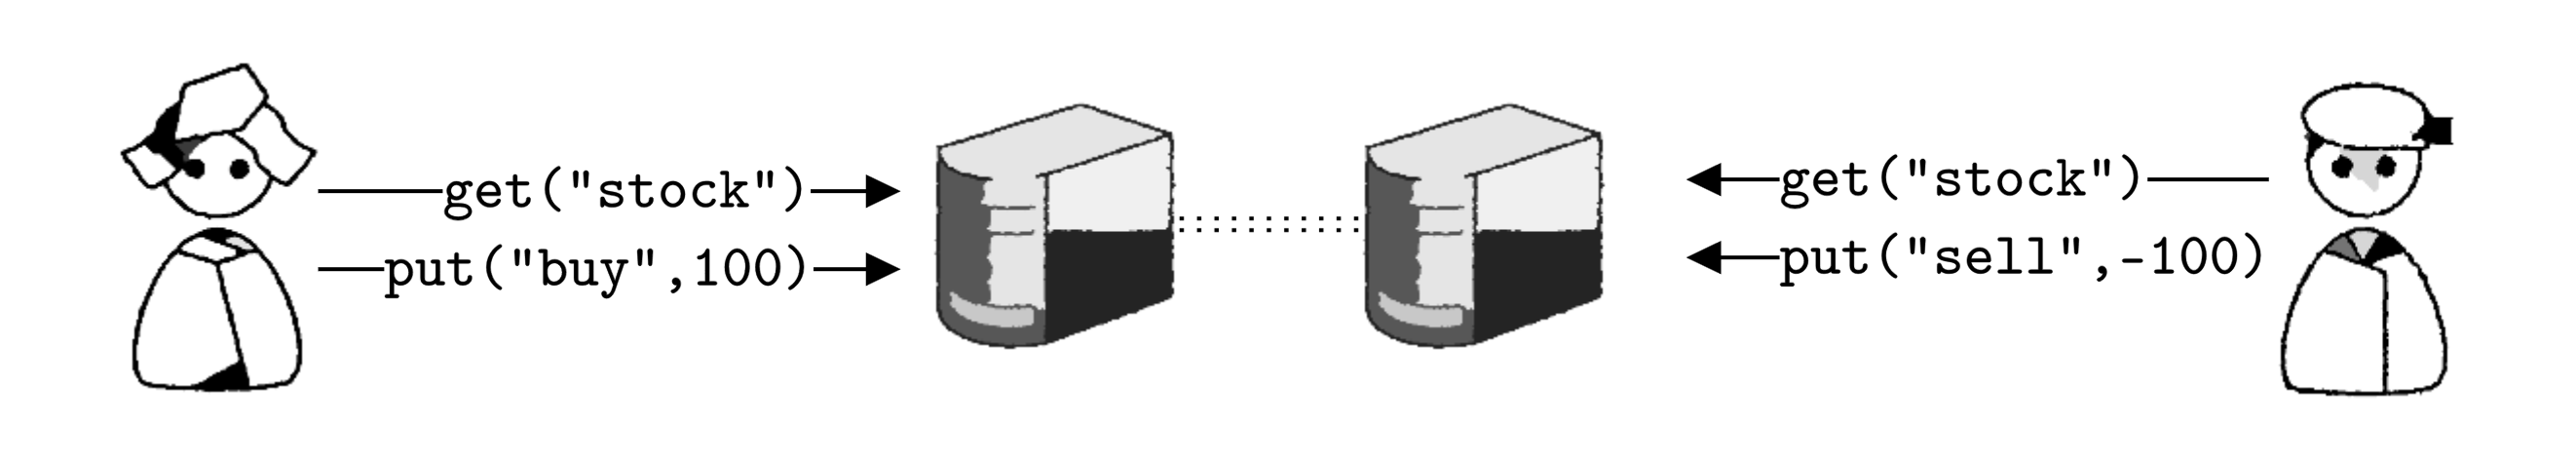
\includegraphics[width=\textwidth]{Sections/trans/stock.png}
    \caption{Two users checking the stock prices and making a trade based on such information.}
    \label{fig:stock_trading}
\end{figure}

\noindent
It is critical that the stock price is consistent through all servers, and 
more important that if any trade fails, the system can recover to a consistent state.

\begin{Def}[Transaction]

    A \textbf{transaction} is a sequence of operations that are treated as a single unit of work.
    A transaction must satisfy the \textbf{ACID} properties:
    \begin{itemize}
        \item \textbf{Atomicity}: A transaction is either fully completed or dropped entirely.
        \item \textbf{Consistency}:  A transaction takes the database from one valid state to another.
        \item \textbf{Isolation}: Transactions must be isolated from each other.
        \item \textbf{Durability}: Once a transaction is committed, it remains so even after system failure.
    \end{itemize}
\end{Def}

\vspace{-0.5em}
\begin{figure}[h]
    \centering 
    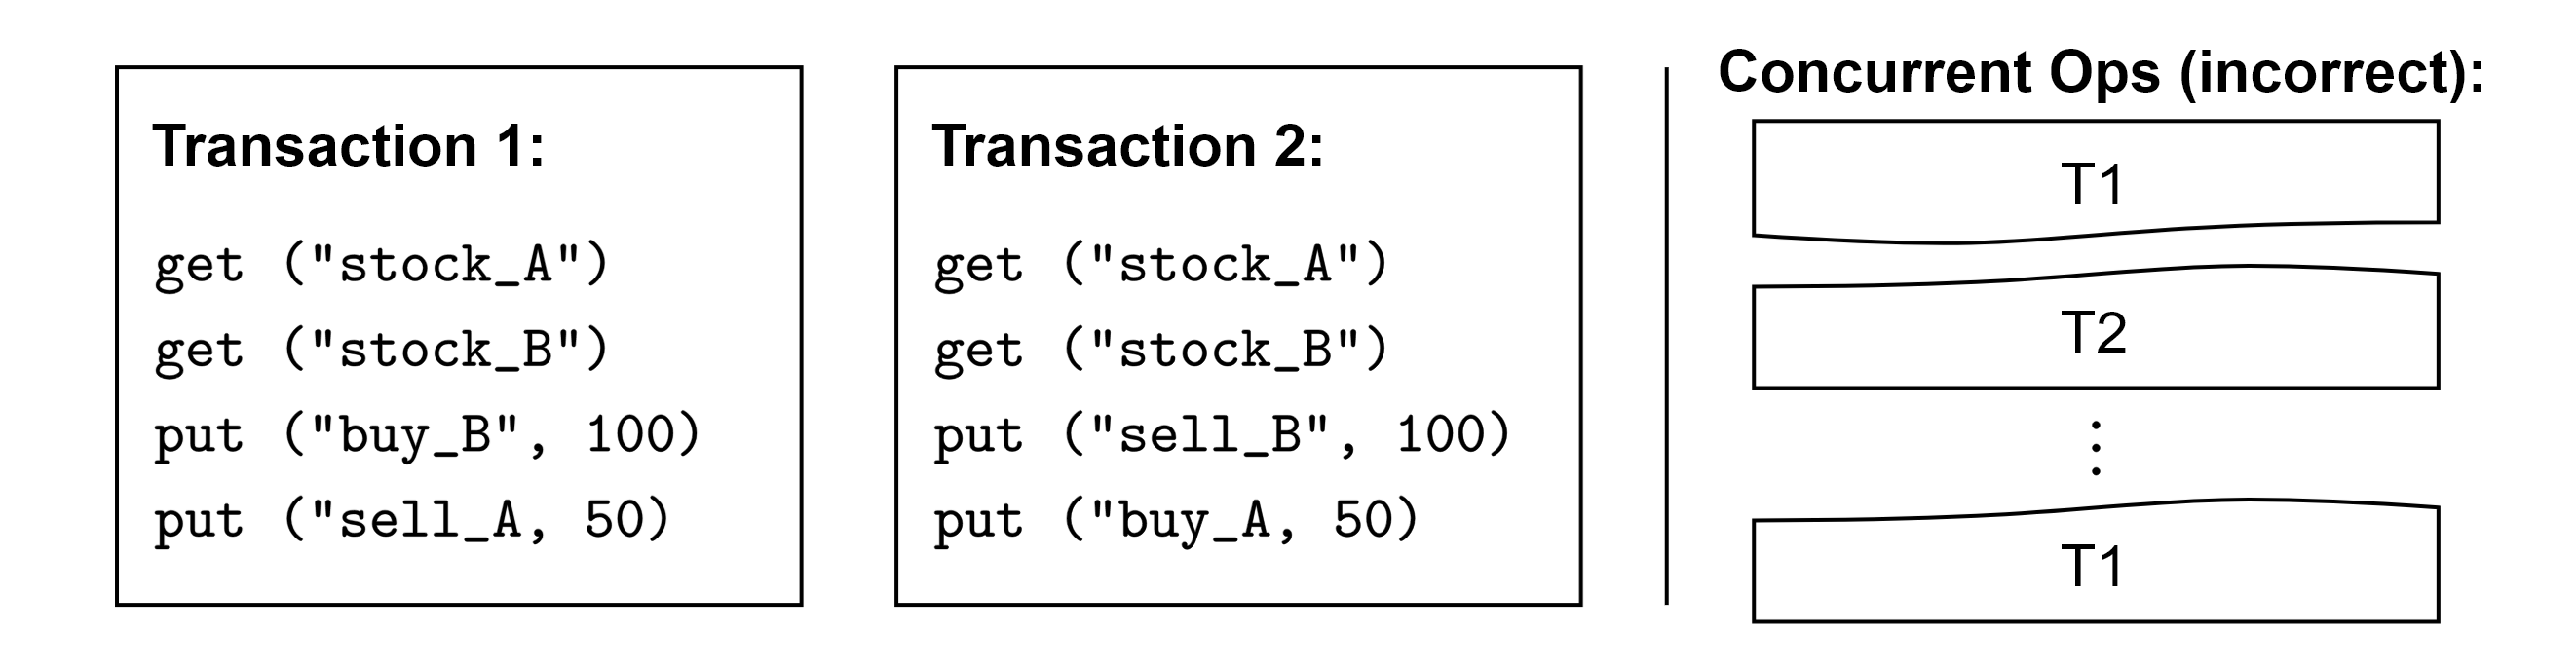
\includegraphics[width=\textwidth]{Sections/trans/stock_2.png}
    \caption{Two transactions which whose operations are interleaved.}
    \label{fig:stock_trading}
\end{figure}

\noindent
Interleaving transactions \textbf{violates the isolation property}. This is problematic in 
Figure (\ref{fig:stock_trading}) as T2's (transaction 2) operations may depend on the server 
state before T1's transaction. Additionally partially completed transactions leave the system in an inconsistent state, violating
\textbf{atomicity}
(e.g., T1's ``buy\_B'' fails, but ``sell\_A'' succeeds).

\newpage

\noindent
We discuss another consistency model which will help us in this settings:
\begin{Def}[Serializability]

    \label{def:serializability}
    
    \textbf{Serializability} is a strong consistency model that ensures the outcome of concurrent transactions is the same as if they were executed in some sequential (serial) order.\\
    
    \noindent
    This differs from \textbf{linearizability}, which focuses on the real-time ordering of individual operations. Serializability instead concerns the logical order of \textbf{entire transactions}, independent of their timing.\\ 

    \noindent
    However, \textbf{strict-serializability} does care about real-time ordering in addition to the logical order of transactions. This implies linearizability, but not vice versa.
    
    \end{Def}

\noindent
We consider the following model to help us preform transactions:
\begin{Def}[Optimistic Concurrency Control (OCC)]

    \textbf{Optimistic Concurrency Control (OCC)} assumes conflicts are rare and proceeds without locking. It follows four main steps:
    
    \begin{itemize}
        \item \textbf{Prepare}: The system reads the transaction request and creates a backup or temporary copy of the state.
        \item \textbf{Modify/Validate}: The transaction modifies the temporary state. Then The system checks whether the transaction is \textbf{serializable}.
        \item \textbf{Commit/Rollback}: If valid, commit; Otherwise, abort transaction and rollback to previous state.
    \end{itemize}
    
    \noindent
    \underline{This only solves \textbf{isolation},} as it does \textbf{not} guarantee atomicity.
    \end{Def}
    \begin{Def}[Transaction Coordinator and Database Servers]

        OCC maintains two necessary components: 
        
        \begin{itemize}
            \item \textbf{Transaction Coordinator (TC)}: The validation server responsible for checking whether a transaction is \textbf{serializable}. It receives requests from clients and responds with either:
            \begin{itemize}
                \item \texttt{OK}: if the transaction is serializable,
                \item \texttt{ABORT}: if it conflicts with prior transactions.
            \end{itemize}
        
            \item \textbf{Database Servers (DB)}: Receives transaction operations, executing it on local state. Then, on \textbf{OK}---commit state, on \textbf{ABORT}---rollback to the previous state.
        
        \end{itemize}        
        \end{Def}
        
    \newpage 

    \noindent
    We consider one model, which where multiple clients interact with one TC.
    \begin{Example}[Centralized OCC]

        Consider these two examples with a single TC and multiple clients on the network line:\\

       \noindent
        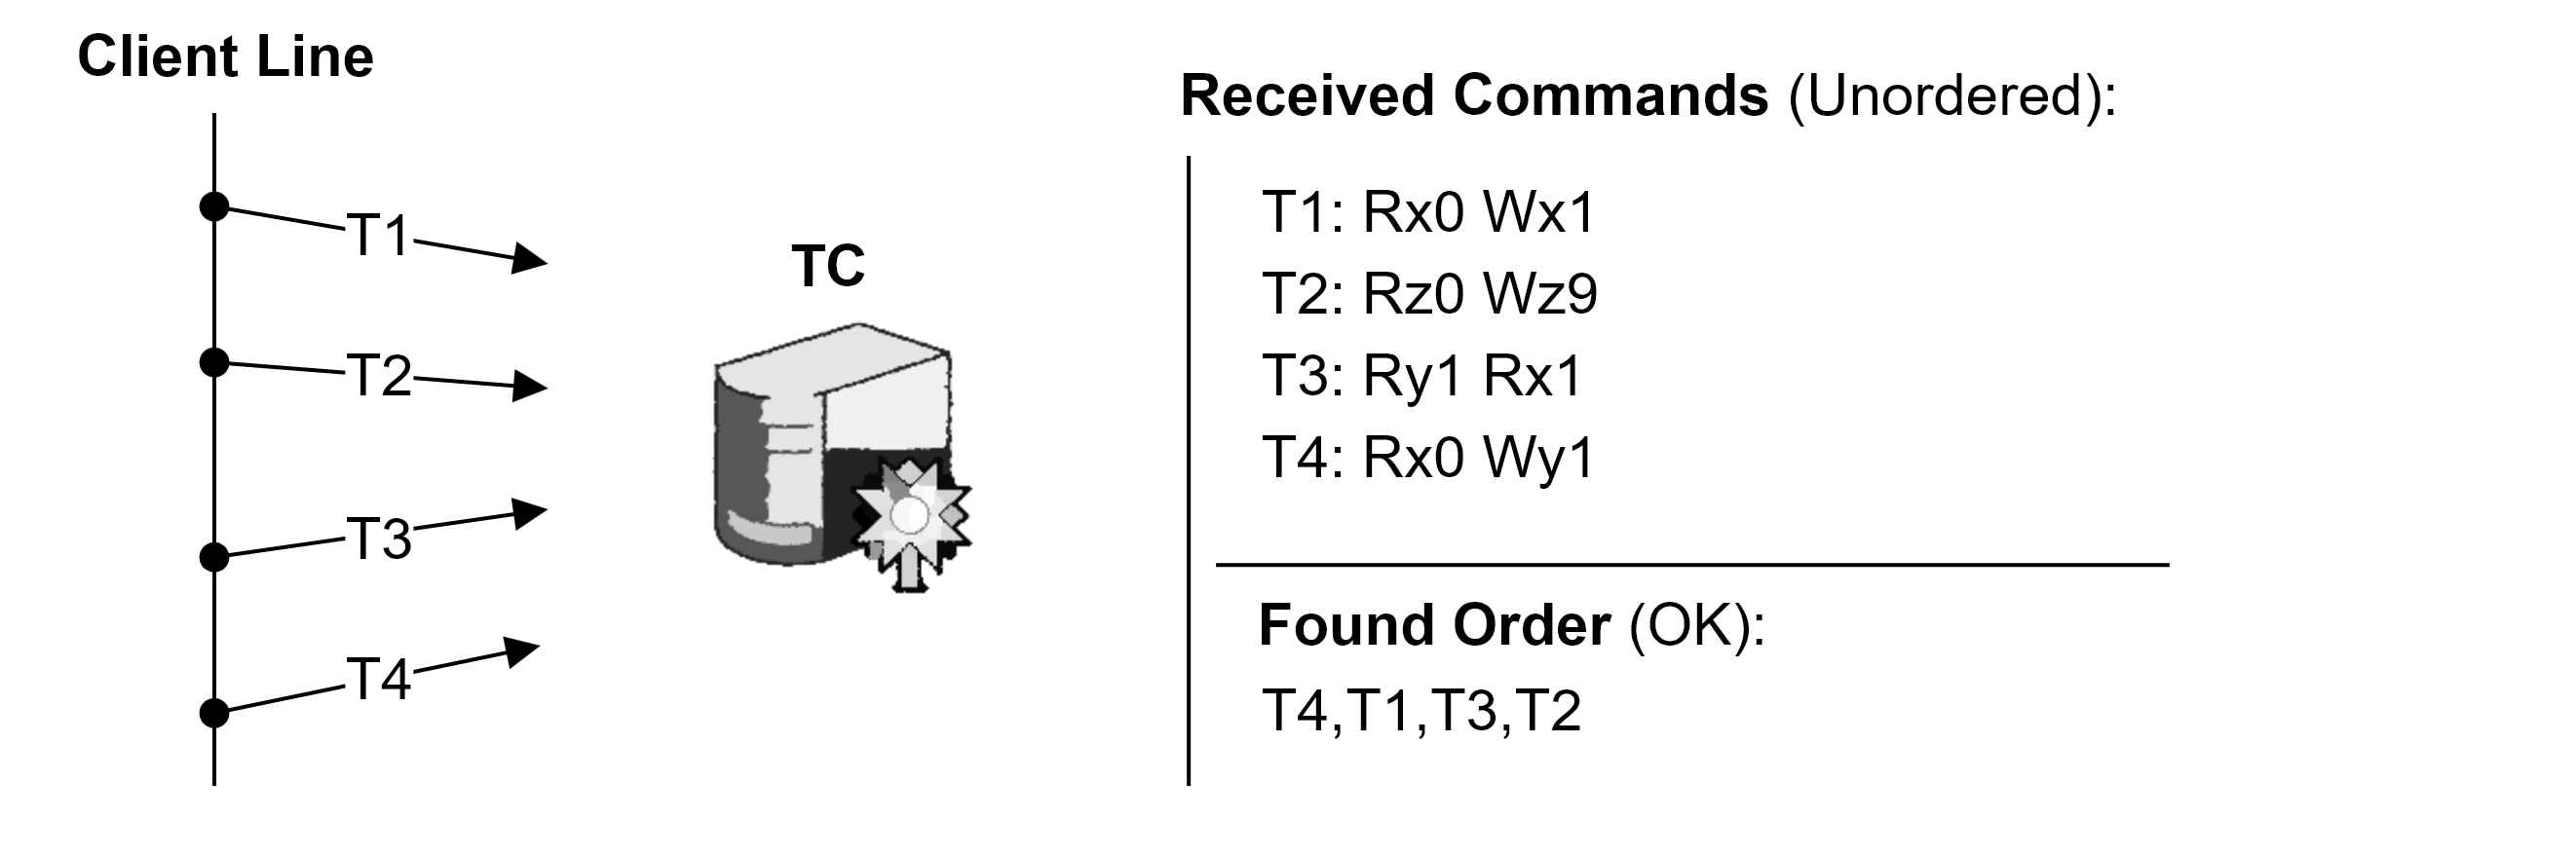
\includegraphics[width=\textwidth]{Sections/trans/central_1.png}
           
        \noindent
        Here, clients on the line send transactions T1--T4 to the TC. The TC then checks the transactions for serializability.
        In this case an order is found (T4,T1,T3,T2), which the TC communicates to the DBs to commit.\\

        \noindent
        \rule{\textwidth}{0.4pt}\\

        \noindent
        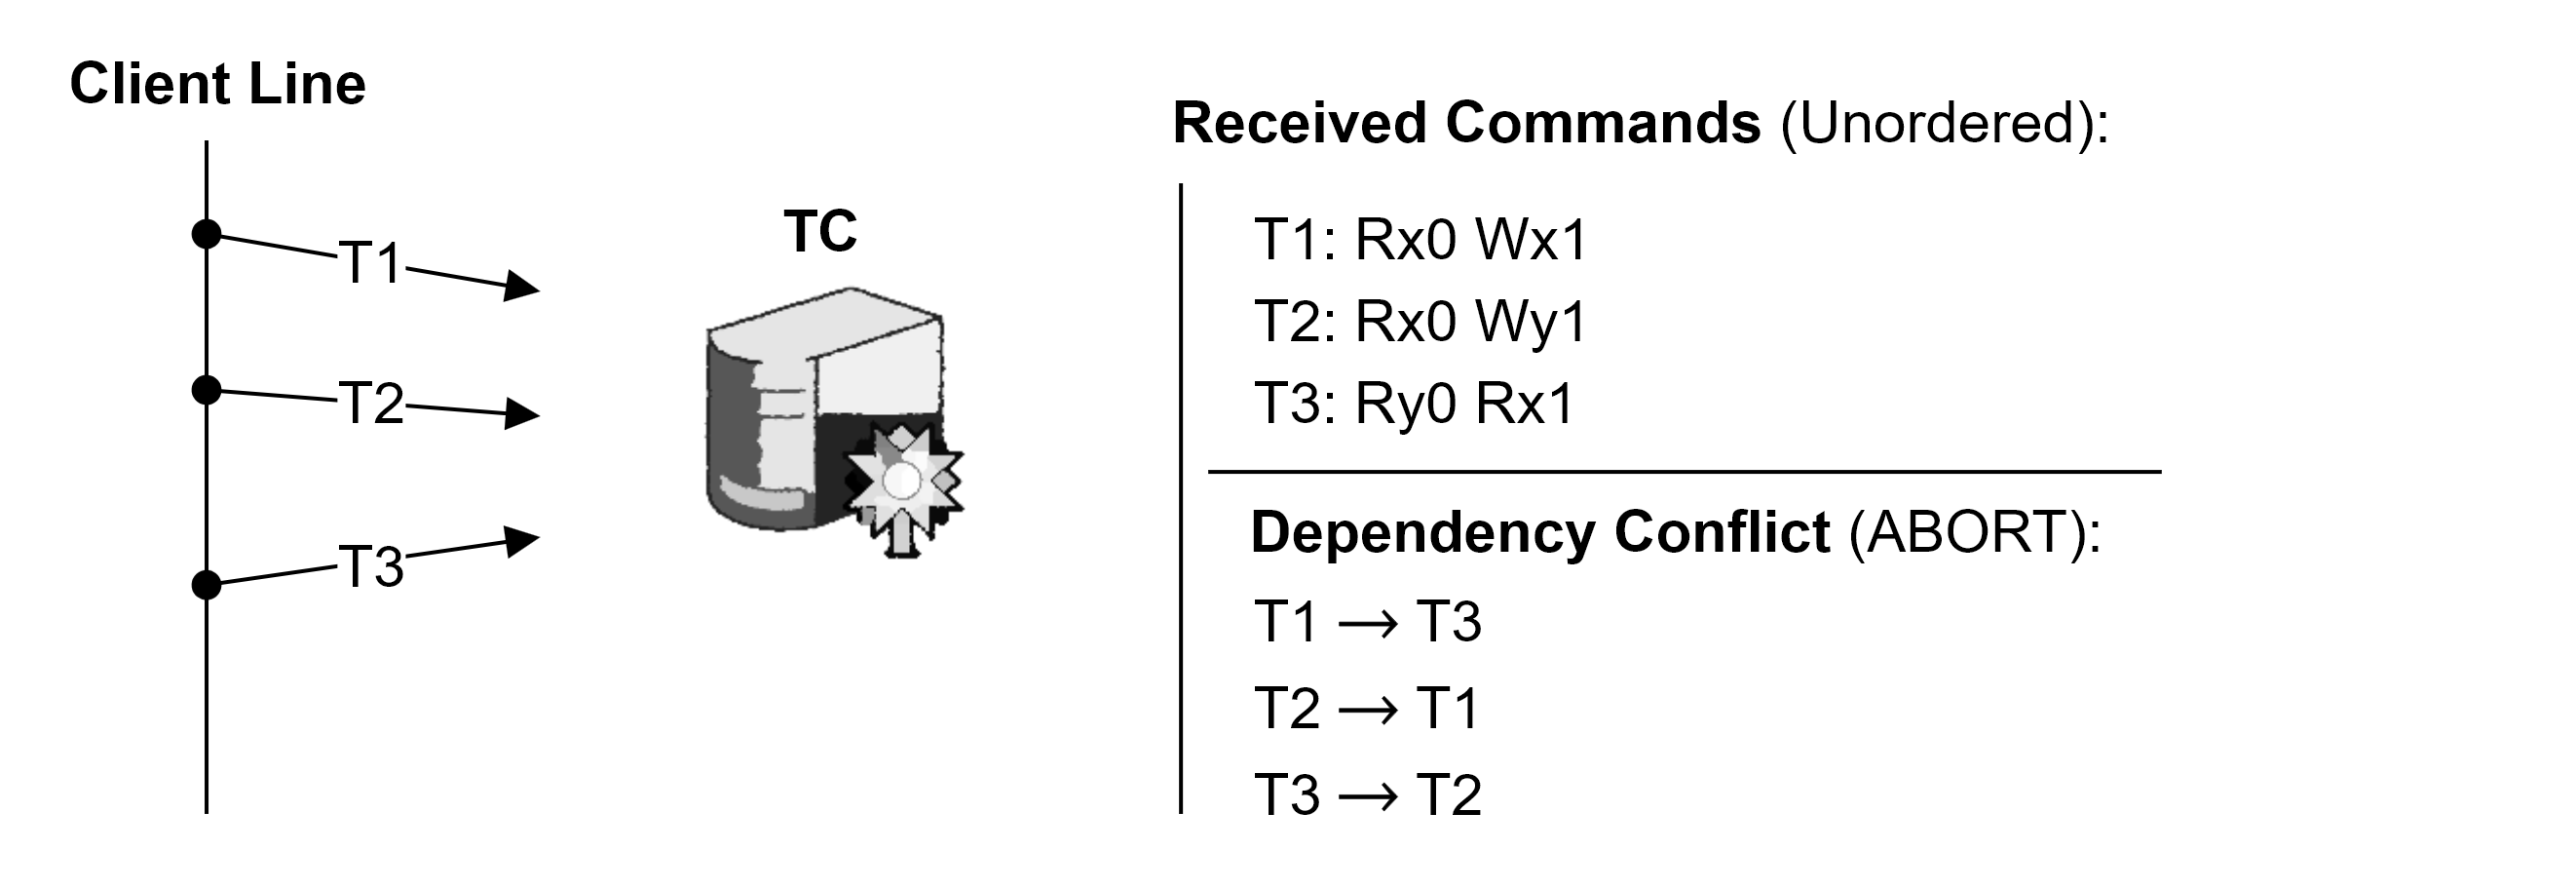
\includegraphics[width=\textwidth]{Sections/trans/central_2.png}

        \noindent
        Here, transaction requests, T1, T2, and T3, do not have a serial order.
        As we build, T1 $\to$ T3 (T1 then T3) makes logical sense. Then T2 $\to$ T3, giving us the order T2 $\to$ T1 $\to$ T3;
        However, it appears T3 must come before T2. This causes a cycle (T2 $\to$ T1 $\to$ T3 $\to$ T2).
        Hence, the TC must must abort all transactions.
    \end{Example}

    \begin{Tip}
    If familiar with \textbf{Directed Acyclic Graphs (DAG)}, one can think of the transactions as nodes and the edges as the dependencies between them.
    If the graph is a DAG, then there is some serial order (OK). If not, then there is a cycle, so we must abort.
    \end{Tip}

    \newpage

    \noindent
    Though we run into an issue when there are multiple TCs.
    \begin{Example}[Distributed OCC]

        Consider two TCs responsible for different parts of our system data.

        \noindent
        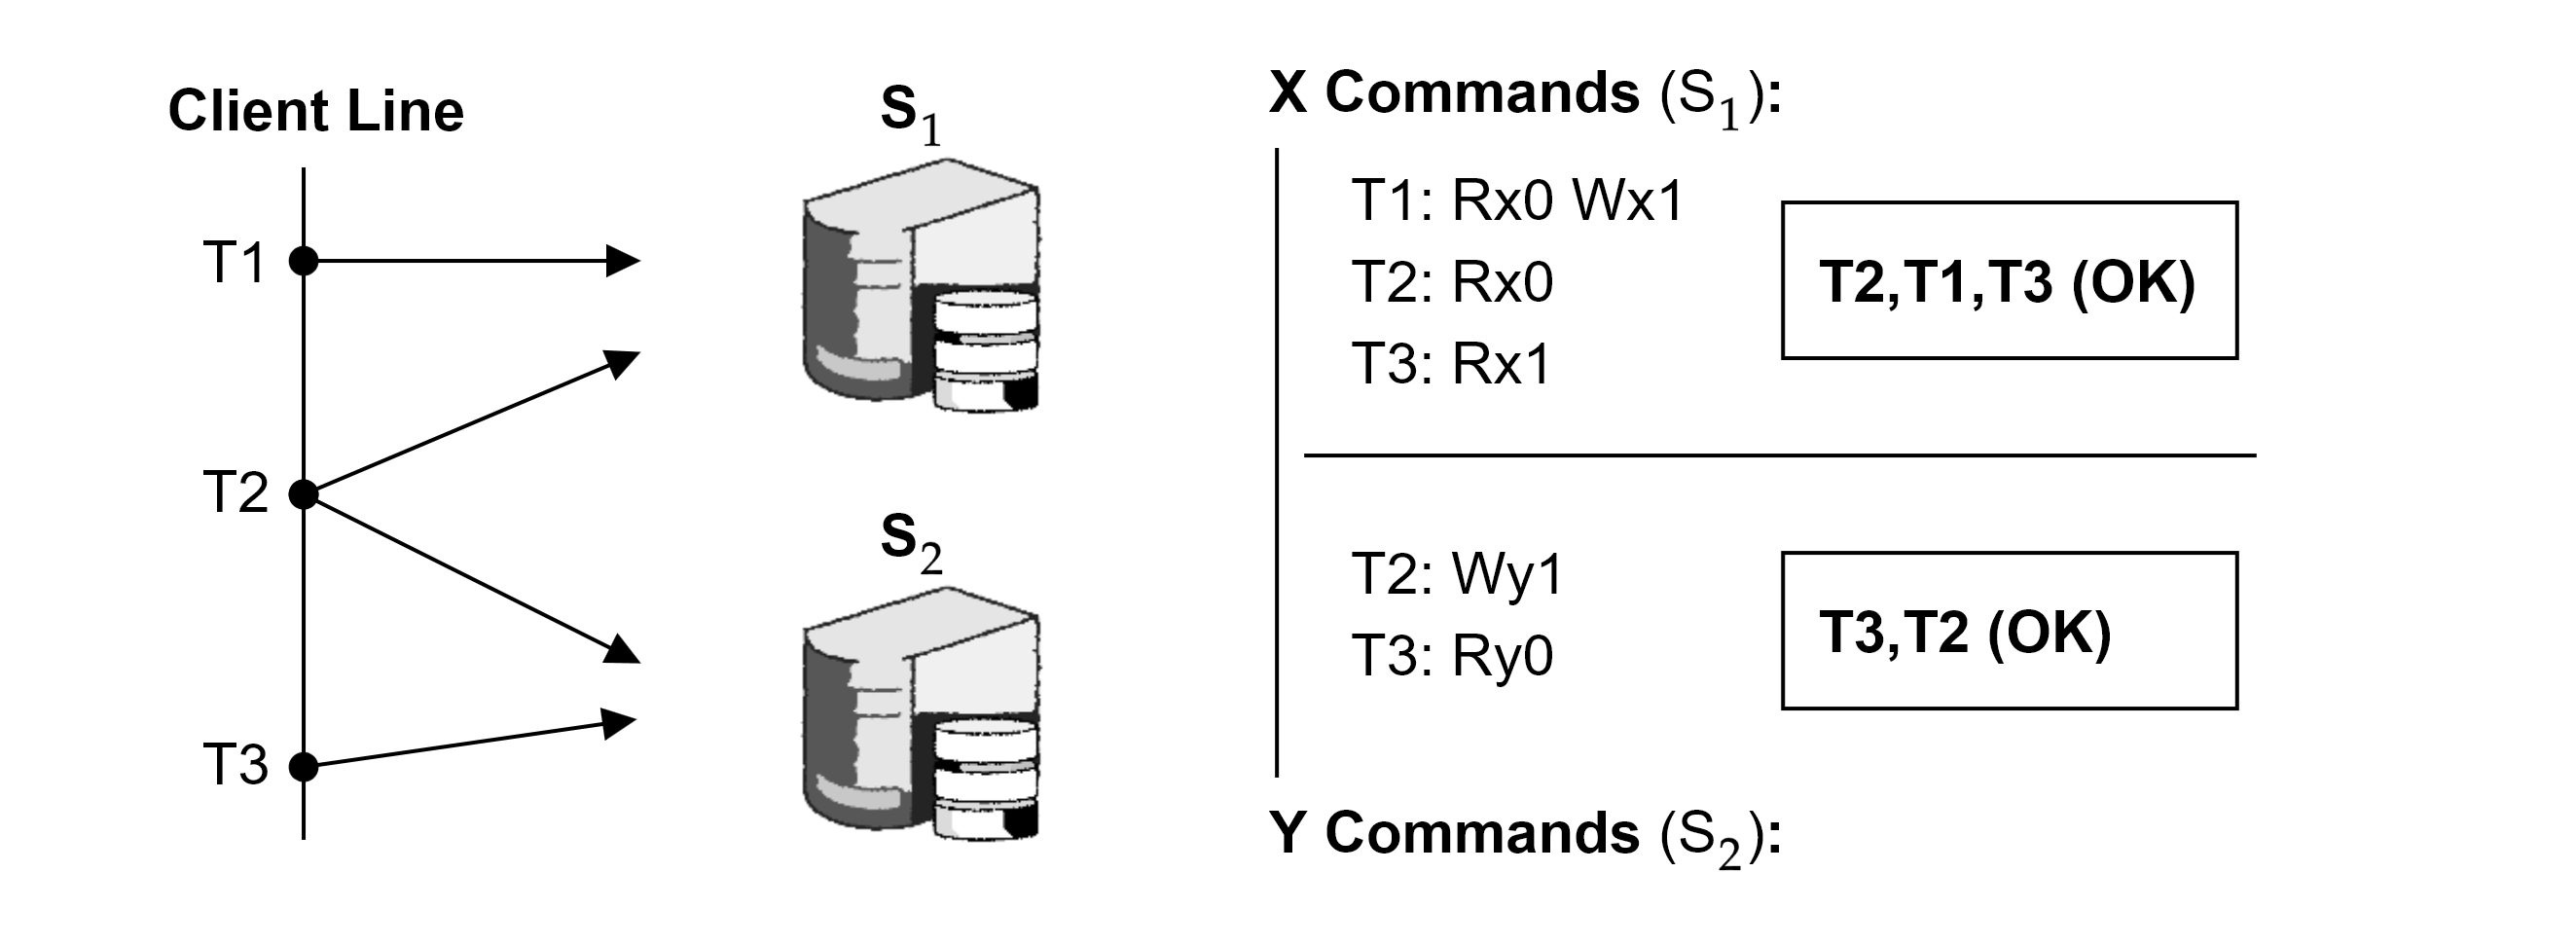
\includegraphics[width=\textwidth]{Sections/trans/central_3.png}

        \noindent
        The problem occurs as TC$_1$ and TC$_2$ pick \textbf{different serial orders} for the transactions.
    \end{Example}
    
\begin{theo}[Timestamping Distributed OCC]

    \textbf{Timestamping} is a method where each transaction is assigned a unique timestamp (ID), which aids
    order agreement between TCs. The downside: \textbf{unnecessary aborts.}
\end{theo}

\begin{Example}[Timestamping Distributed OCC]

    \vspace{-1em}
    \noindent
    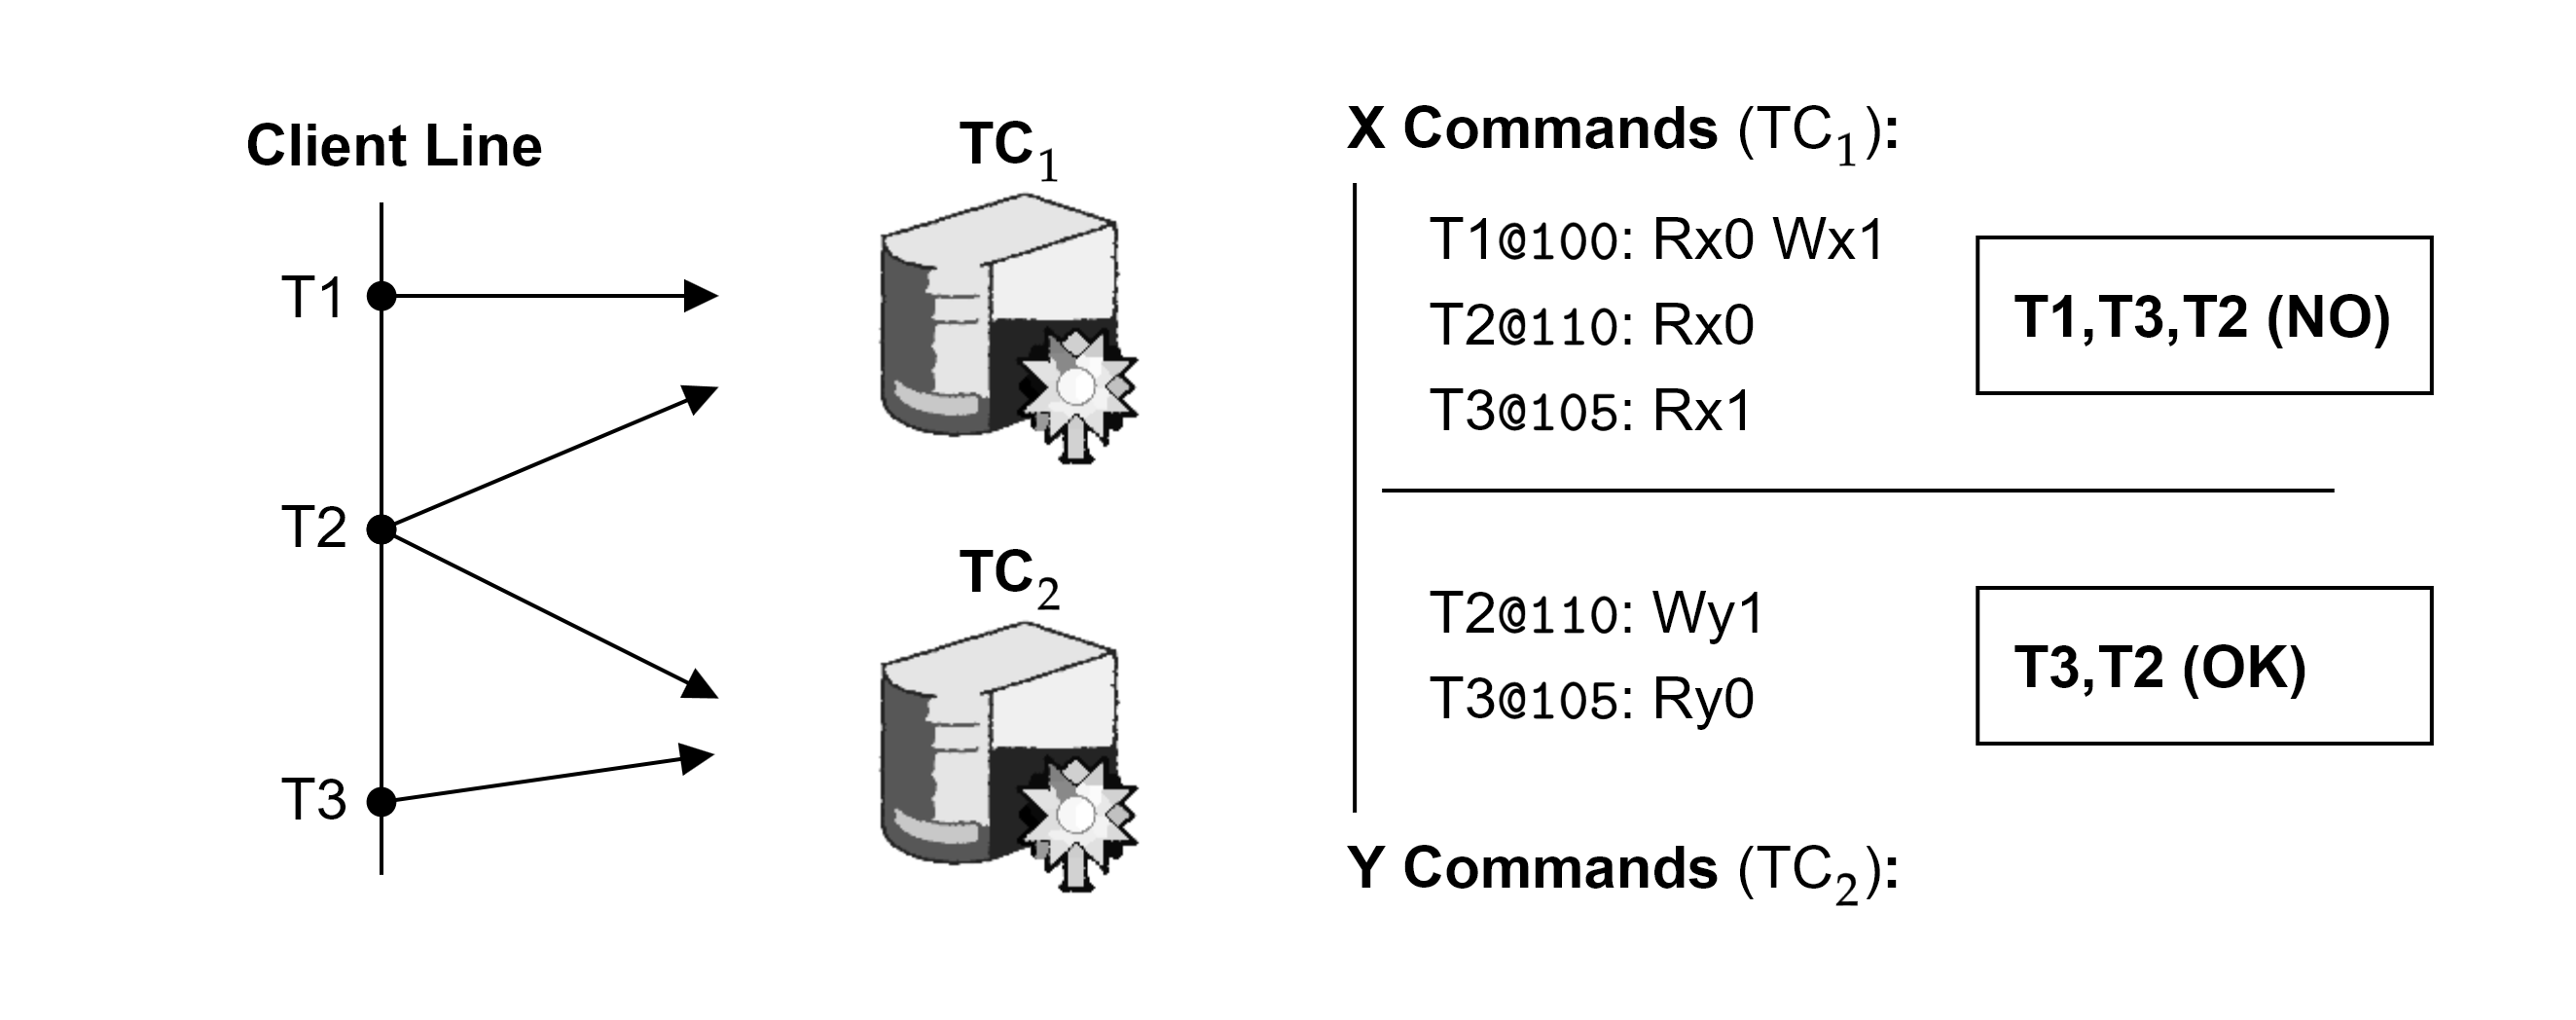
\includegraphics[width=\textwidth]{Sections/trans/central_4.png}

    \noindent
    \underline{\textbf{Timestamps (@\#) only serve as IDs.}} Here TC$_2$ OKs the order (T3,T2). TC$_1$ sees this,
    enforces the order, but is not able to serialize (T1,T3,T2). Hence, it aborts (NO).
    \end{Example}

    \newpage 

\subsection{Two-Phase Commit (2PC)}
\noindent
We introduce another method to help us with this problem, though it \textbf{does not ensure isolation}:

\begin{Def}[Two-Phase Commit (2PC)]

    \underline{\textbf{Two-Phase Commit (2PC)} ensures \textbf{atomicity}.}
    The client sends the transactions to the DBs (participants). There after, the client tells the TC start the commit process, involving two phases:
    
    \begin{itemize}
        \item \textbf{Prepare Phase}: The coordinator sends a prepare request to all DBs; Each respond:
        \begin{itemize}
            \item \texttt{YES}: if it can commit the transaction.
            \item \texttt{NO}: if it cannot commit the transaction.
        \end{itemize}
        \item \textbf{Commit Phase}: If all voted \texttt{YES}, the coordinator sends a \texttt{COMMIT} request to all DBs. If any participant voted \texttt{NO}, the coordinator sends an \texttt{ABORT}.
        The TC then responds to the client with the final outcome of the transaction.
    \end{itemize}
\end{Def}

\begin{figure}[h]
    \centering
    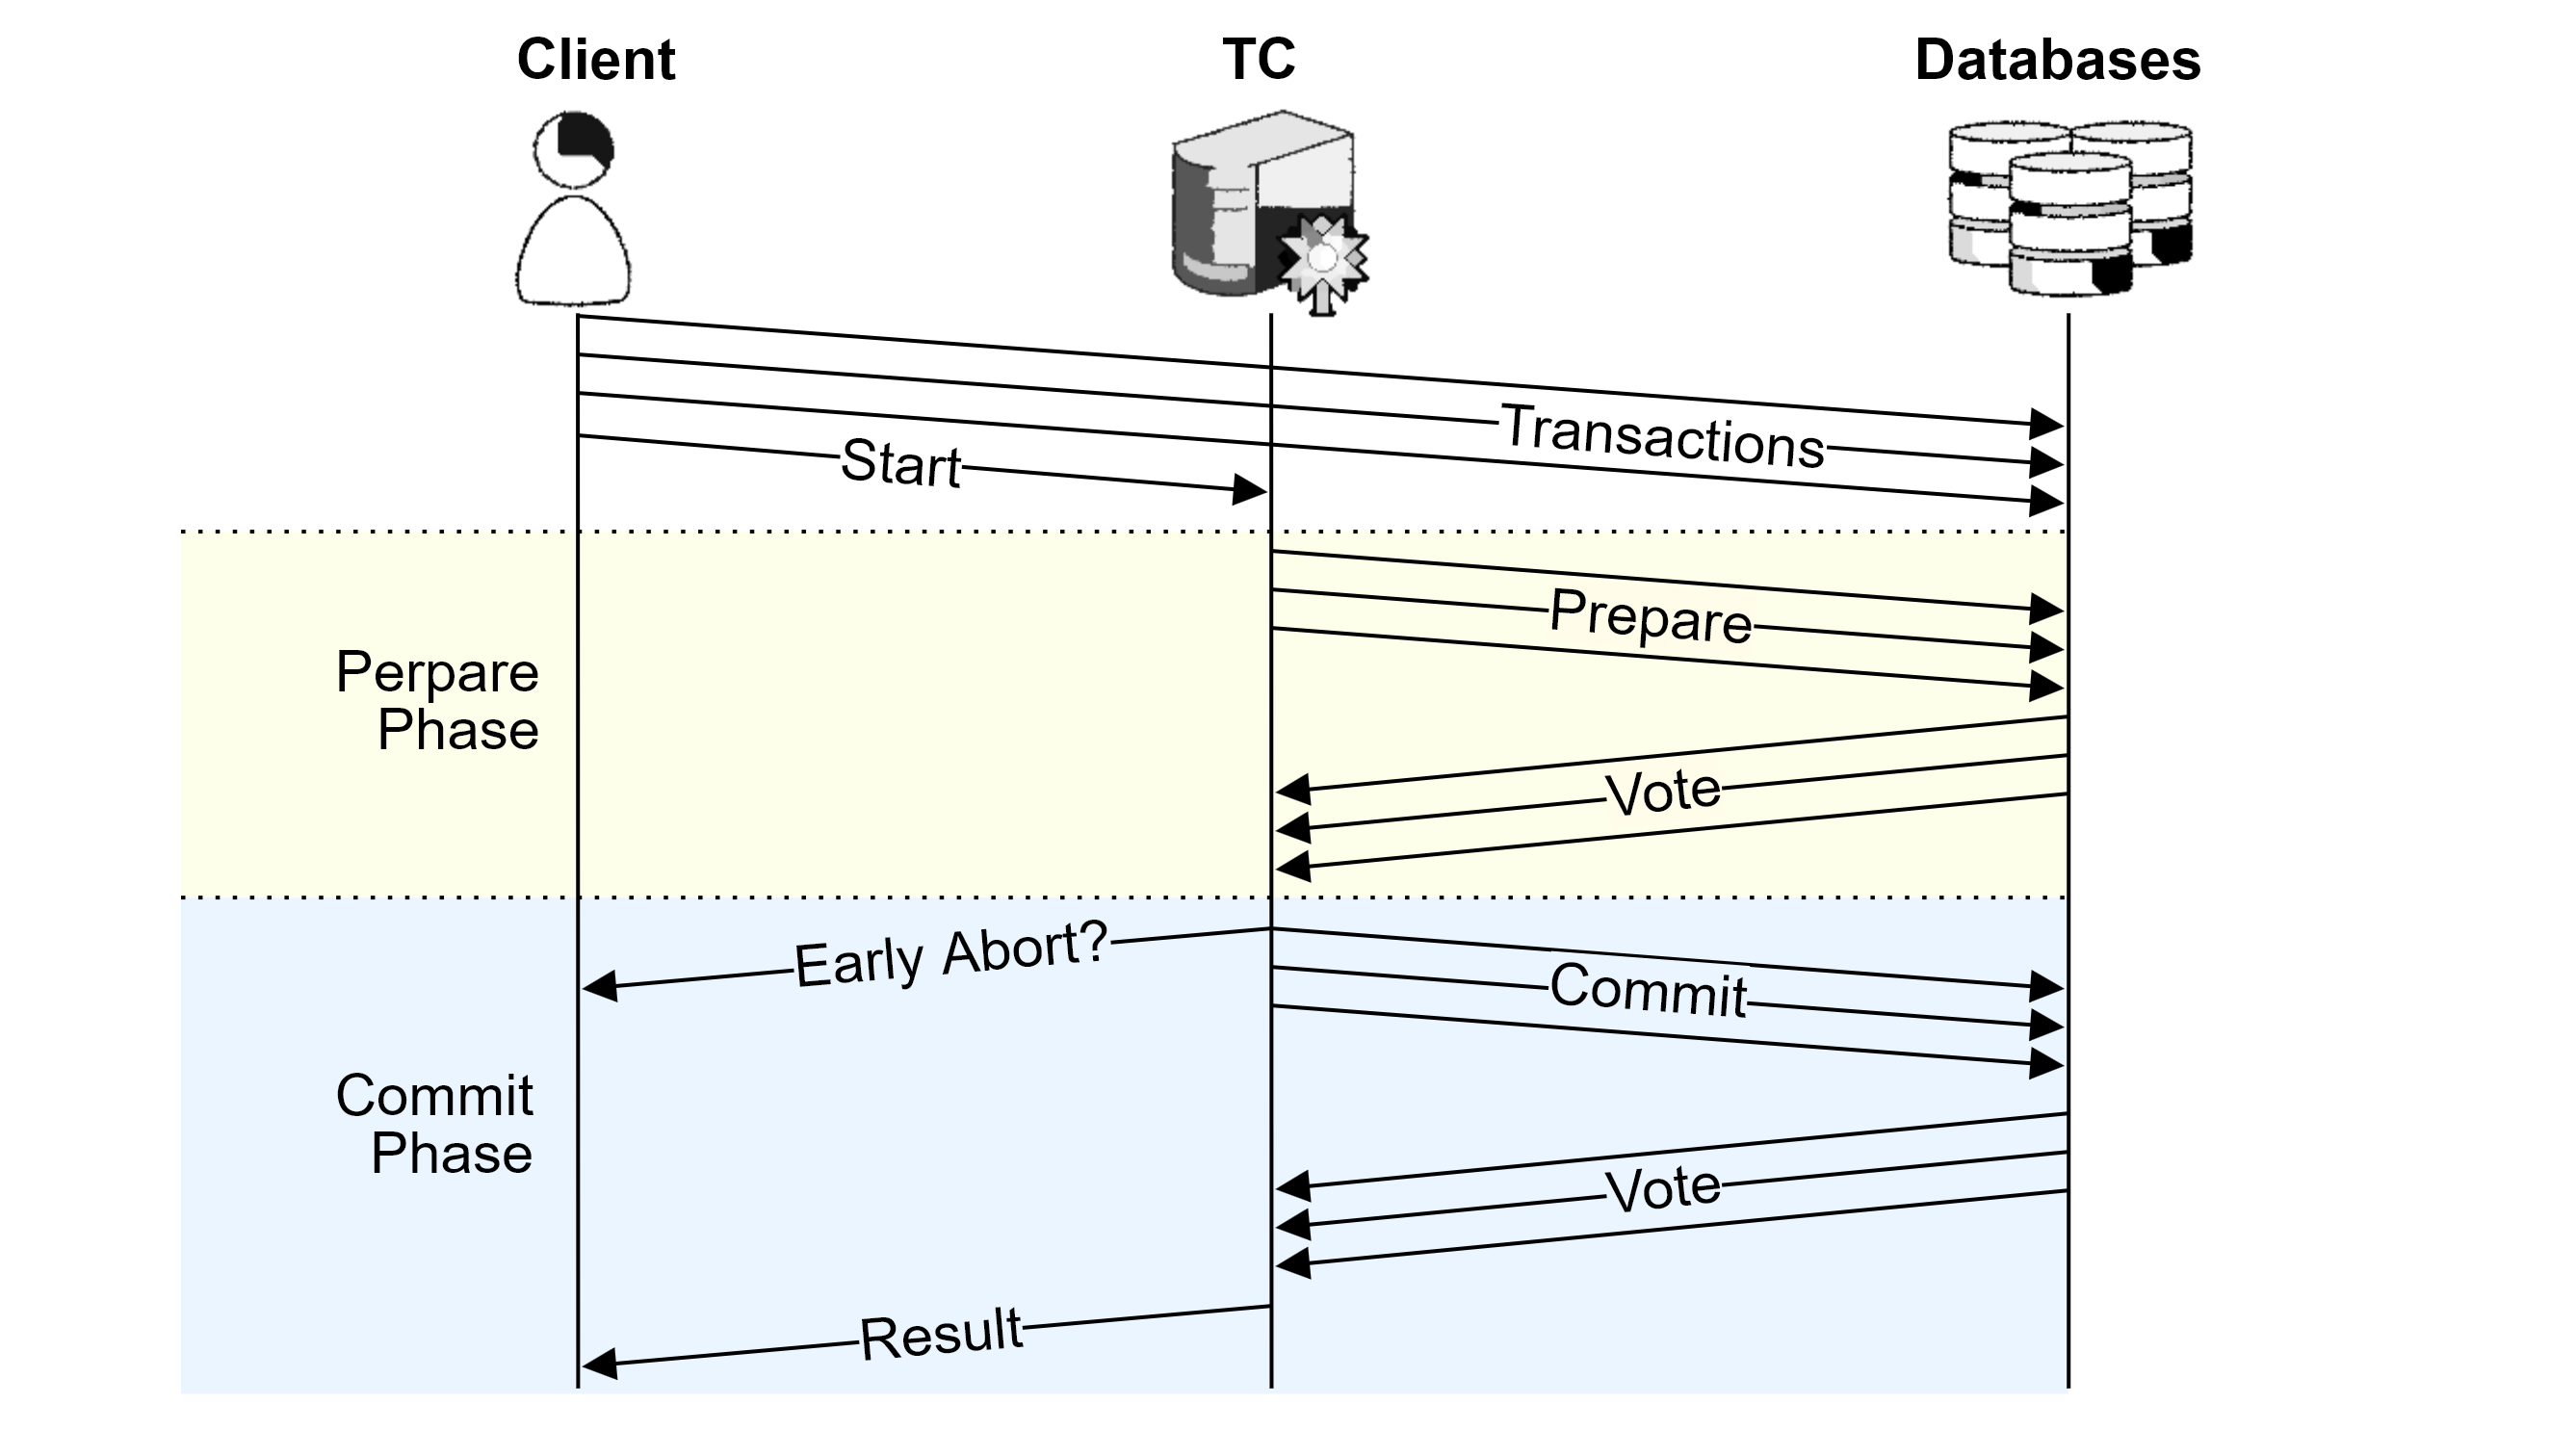
\includegraphics[width=\textwidth]{Sections/trans/2PC.png}
    \caption{Two-Phase Commit (2PC) process. The client sets up the transaction with the TC and DBs. Then, the TC starts the 
    commit process, starting with the prepare phase, and then ends with the commit phase.}
    \label{fig:2pc}
\end{figure}

\newpage 

\noindent
Though there is a pitfall with this method:

\begin{Def}[2PC Blockout]

   In most cases if there's a timeout the TC or DBs will abort the transaction.
   However, if the TC times out after a DB has voted \texttt{YES}, the DB is left in an uncertain state, 
   and must \textbf{wait} for the TC to respond.
\end{Def}

\noindent
\resizebox{\textwidth}{!}{%
\renewcommand{\arraystretch}{1.6}
\begin{tabular}{|p{5cm}|p{6cm}|}
    \hline
    \rowcolor{Black} \multicolumn{2}{|c|}{\textcolor{white}{\large \textbf{Preparation Phase}}} \\
    \hline
    \rowcolor{OliveGreen!10} \textbf{\large Case} & \textbf{\large Action} \\
    \hline
    TC timeout for yes/no vote & \large \textbf{Abort} — transaction coordinator did not receive votes in time. \\
    \hline
    DB timeout for prepare & \large \textbf{Abort} — database did not receive prepare request in time. \\
    \hline

    \rowcolor{Black} \multicolumn{2}{|c|}{\textcolor{white}{\large \textbf{Commit Phase}}} \\
    \hline
    \rowcolor{OliveGreen!10} \textbf{\large Case} & \textbf{\large Action} \\
    \hline
    DB timeout for commit/abort and DB voted NO & \large \textbf{Abort} — since DB already voted NO, it's safe to abort. \\
    \hline
    DB timeout for commit/abort and DB voted YES & \large \textbf{Block} — DB must wait for TC decision to preserve atomicity. \\
    \hline
\end{tabular}
}

\begin{Def}[2PC Persistent \& Volatile State]

    In the Two-Phase Commit (2PC) protocol, both the Transaction Coordinator (TC) and Database (DB) participants must persist critical information to recover correctly after a crash.

    \begin{itemize}
        \item \textbf{Database (DB):}
        \begin{itemize}
            \item Must persist the result of any vote (\texttt{YES} or \texttt{NO}).
            \item If the DB voted \texttt{YES} and then crashes, upon recovery it must contact the TC to learn the final decision (\texttt{COMMIT} or \texttt{ABORT}).
        \end{itemize}

        \item \textbf{Transaction Coordinator (TC):}
        \begin{itemize}
            \item Must persist the result of any vote and the final decision (\texttt{COMMIT} or \texttt{ABORT}).
            \item If the TC crashes, it must resume the commit protocol from where it left off.
        \end{itemize}
    \end{itemize}

\end{Def}





\newpage 
\subsection{Three-Phase Commit (3PC)}
\noindent
2PC's main problem was \textbf{availability}. We can fix this by adding an additional phase:
\begin{Def}[Three-Phase Commit (3PC)]

    \textbf{Three-Phase Commit (3PC)} is an extension of 2PC that adds a third phase to avoid blocking in case of failures:
    
    \begin{itemize}
        \item \textbf{CanCommit Phase}: The coordinator sends a \texttt{CANCOMMIT} request to all participants. Each participant responds with either \texttt{YES} or \texttt{NO}.
        \item \textbf{PreCommit Phase}: If all participants respond with \texttt{YES}, the coordinator sends a \texttt{PRECOMMIT} request to all participants. Participants prepare to commit sending back an acknowledgment (\texttt{ACK}).
        \item \textbf{DoCommit Phase}: If all participants \texttt{ACK} the precommit, the coordinator sends a \texttt{COMMIT} request. Otherwise, it sends an \texttt{ABORT} request.
    \end{itemize}
\end{Def}

\begin{theo}[3PC Non-Blocking Nature \& Self-Resolution]

    The reason this fixes the blocking issue in 2PC lies within the \texttt{PRECOMMIT} phase.
    In regular 2PC, if a DB votes \texttt{YES} it must wait for the TC to respond as it is uncertain whether another DB 
    has committed or not.

    In 3PC, such DB need not worry, as no other DB can commit until the TC sends a \texttt{PRECOMMIT} request. Henceforth,
    DBs can safely either terminate or resolve between themselves that if everyone else has the \texttt{PRECOMMIT} request, they can commit.
\end{theo}

\begin{theo}[3PC Persistent \& Volatile State]

    Both the TC and DBs may crash at any time, for which they must persist the state of the transactions.
    Though it is fully possible for the TC to only persist the original transaction request, and instead 
    query \underline{\textbf{all}} DBs for their state to recover the transaction. 
\end{theo}    

\begin{theo}[3PC Tradeoffs]

    \begin{itemize}
        \item ($-$) If the network becomes partitioned, inconsistencies may arise within self-resolution.
        \item ($-$) Adds another round trip to the commit process (3 in total).
        \item ($+$) Removes the blocking issue of 2PC, as the TC can always recover from a crash. 
    \end{itemize}
\end{theo}


\newpage 

\noindent
Below is a diagram of the 3PC process:
\begin{figure}[h]
    \centering
    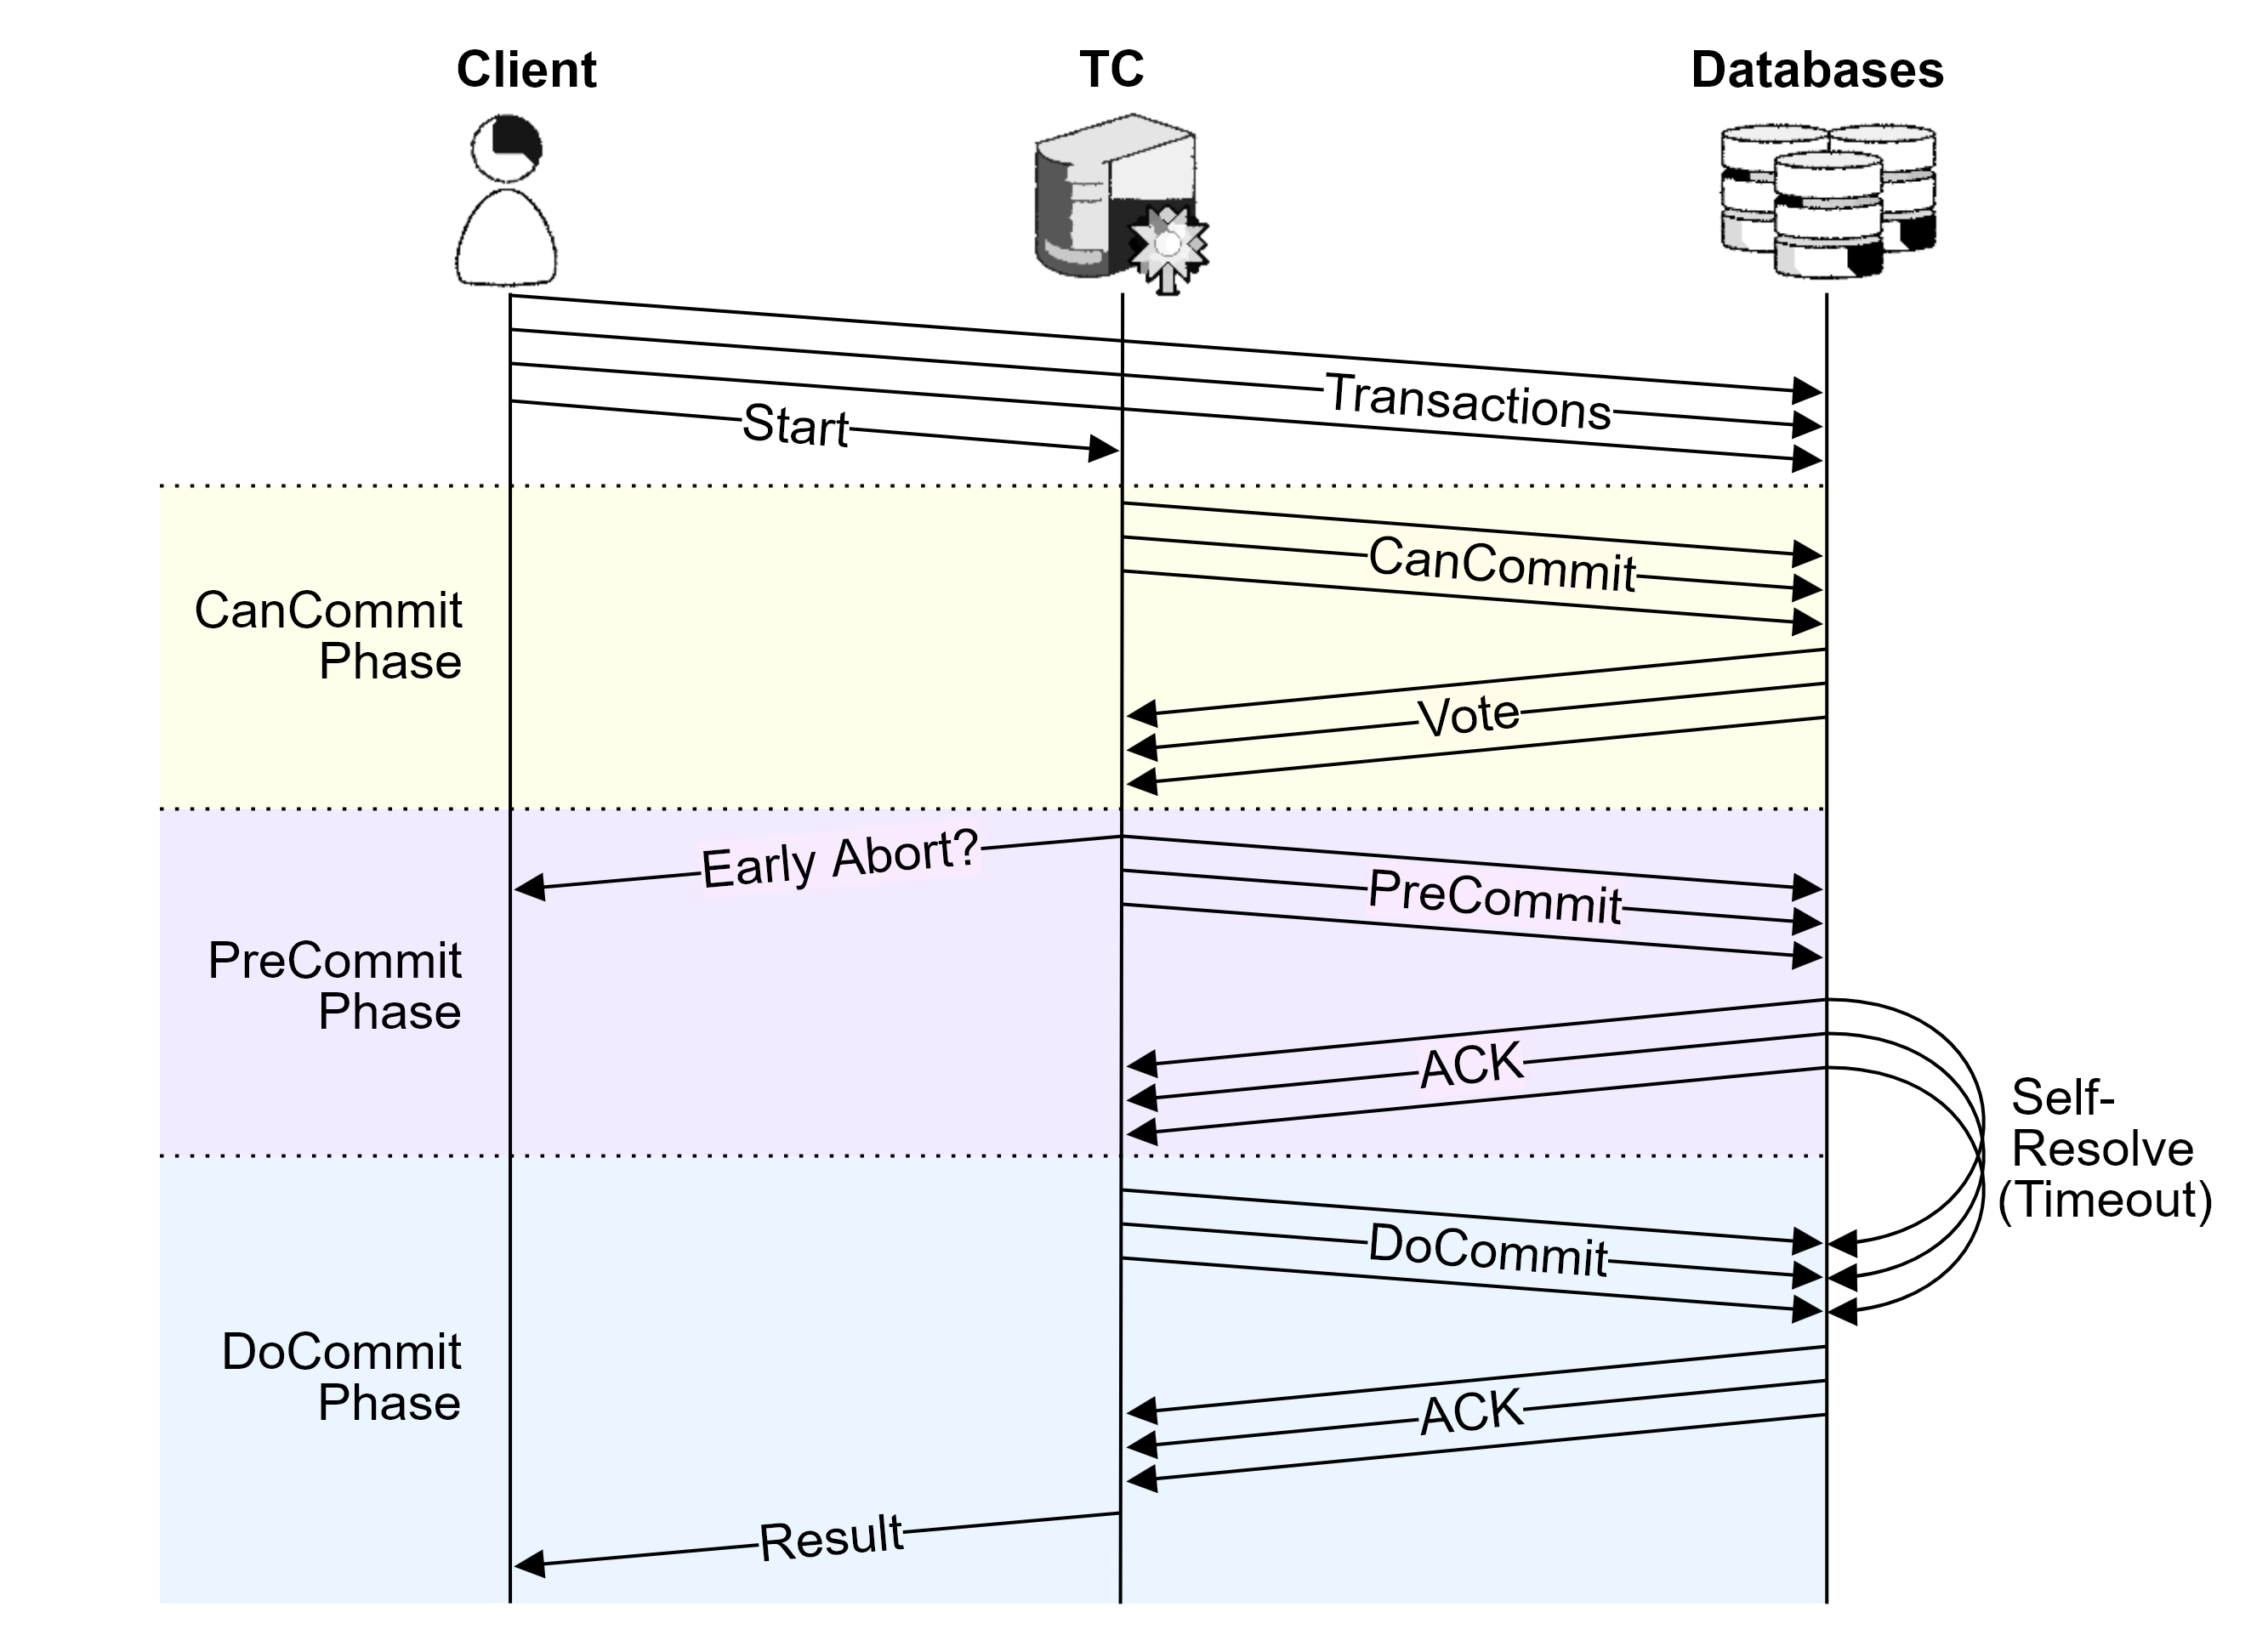
\includegraphics[width=\textwidth]{Sections/trans/3PC.png}
    \caption{Three-Phase Commit (3PC) protocol message flow. The transaction progresses through three phases: \textbf{CanCommit}, where participants vote; \textbf{PreCommit}, where participants acknowledge readiness to commit; and \textbf{DoCommit}, where the final decision is executed. The TC may decide to abort if it recieved a \texttt{NO} vote, or failed to \texttt{ACK} during \texttt{PreCommit}. In the event of coordinator failure, participants may invoke \textbf{Self-Resolve} after a timeout, based on whether they received a \texttt{PreCommit} message, ensuring non-blocking recovery.
    \textbf{Note:} The Databases do not communicate with the client after resolution, though this could depend on the implementation.}
    \label{fig:3pc}
\end{figure}

\noindent
We briefly go over OCC's opposition:
\begin{Def}[Pessimistic Concurrency Control (PCC)]

    \textbf{Pessimistic Concurrency Control} assumes conflicts are likely and prevents them by acquiring locks before any data access.
    It then preforms actions directly on shared data, ensuring \textbf{serializability and isolation}. The locks are released after the transaction is completed.
  \end{Def}
  